\documentclass[]{beamer}

\usetheme{Antibes}
\usecolortheme{beaver}
\usefonttheme{professionalfonts}
\setbeamercolor{block title}{bg=red!30,fg=black}

\usepackage{pgfpages}
\usepackage[italian]{babel} 
\usepackage[T1]{fontenc}
\usepackage[utf8x]{inputenc}
\usepackage{graphicx}
\usepackage{xcolor}
\usepackage{float}
\usepackage{subfig}
\usepackage[autoplay]{animate}
\usepackage{tikz}
\usepackage{pgfplots}
\usepackage{tikz-3dplot}
\usepackage[mode=image|tex]{standalone}

% New operators
\DeclareMathOperator*{\atan2}{atan2}            % Atan2 
\DeclareMathOperator*{\asin}{asin}              % Asin
\DeclareMathOperator*{\sgn}{sgn}                % Sgn
\DeclareMathOperator*{\diag}{diag}              % Diag

\setbeamercovered{dynamic}

\pgfdeclareimage[height=1cm]{logo_unipd}{images/unipd}
\pgfdeclareimage[height=2cm]{logo_dei}{images/dei}
%\logo{\pgfuseimage{logo_unipd}}
\titlegraphic{\pgfuseimage{logo_dei}}

\title[]{Model identification and flight control design for the Prometheus mapping drone}
\author[Nicola Dal Lago]{ Nicola Dal Lago}
\date[10 ottobre 2016]{10 ottobre 2016}
\institute[DEI Unipd]{Corso di Laurea Magistrale in Ingegneria dell'Automazione\\ Dipartimento di Ingegneria dell'Informazione}

\begin{document}
\frame{\titlepage}


	\section{Introduzione}
	
	\begin{frame}{Prometheus mapping drone}
		\centering	
		\begin{columns}
			\begin{column}{.5\textwidth}
				\centering
				\begin{figure}
					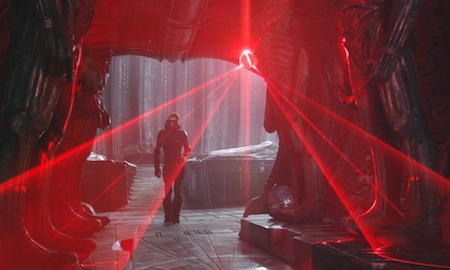
\includegraphics[scale=0.31]{images/prometheus_film.jpg}
				\end{figure}
			\end{column}
			\begin{column}{.5\textwidth}
				\centering
				\begin{block}{Scopo del progetto}
					Realizzazione di un UAV per navigazione e mappatura 3D in autonomo
				\end{block}
			\end{column}
		\end{columns}
		\begin{block}{Progetto diviso in 3 parti:}
			\begin{itemize}
				\item[1] Design e costruzione della parte meccanica
				\item[2] \textcolor{red}{Modello matematico, system identification, traiettorie e controllo} 
				\item[3] Algoritmi di navigazione e mapping
			\end{itemize}
		\end{block}
	\end{frame}
	
	\begin{frame}{Design}
		\centering
		\begin{columns}
			\begin{column}{.5\textwidth}
				\centering
				\begin{figure}
					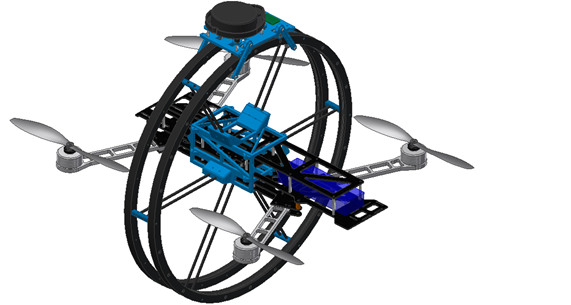
\includegraphics[scale=0.35]{images/render1.png}
				\end{figure}
			\end{column}
			\begin{column}{.5\textwidth}
				\centering
				\begin{itemize}
					\item Telaio di un quadricottero standard 
					\item Uso di un sensore laser Lidar, mapping in 2D
					\item Aggiunta di una piattaforma rotante per mapping in 3D
				\end{itemize}
			\end{column}
		\end{columns}
	\end{frame}
	
	
	\section{Modello matematico}
	
	\begin{frame}{Modello matematico}
		\centering
		Cinematica di Newton-Eulero
		\begin{equation*}
			\begin{bmatrix}
				\mathbf{f}        \\
				\boldsymbol{\tau}
			\end{bmatrix}
			=
			\begin{bmatrix}
				m \cdot I_{3} & \mathbf{0} \\
				\mathbf{0}^T          & I_{cm}
			\end{bmatrix}
			\begin{bmatrix}
				\mathbf{\ddot{x}_B}         \\
				\boldsymbol{\dot{\omega}_B}
			\end{bmatrix}
			+
			\begin{bmatrix}
				\mathbf{0}                                                      \\
				\boldsymbol{\omega_B} \times I_{cm} \cdot \boldsymbol{\omega_B}
			\end{bmatrix}
		\end{equation*}
		\begin{columns}
			\begin{column}{.55\textwidth}
				\centering
				\begin{figure}
					\includestandalone[scale=0.5]{standalone/quadrotor}
				\end{figure}
			\end{column}
			\begin{column}{.55\textwidth}
				\centering
				\begin{align*}
					\mathbf{f}_i(t) &= a_{f,i}\Omega_i^2\mathbf{n}_i = a_{f,i}\Omega_{max, i}^2 u_i(t)^2\mathbf{n}_i \\
					\boldsymbol{\tau}_i(t) &= -\sgn(\Omega_i)b_{f,i}\Omega_{max,i}^2u_i(t)^2\mathbf{n}_i \\
					u_i(t) &\approx \frac{1}{\tau_i s+1}u_{in,i}(t)
				\end{align*}
			\end{column}
		\end{columns}
	\end{frame}
	
	\begin{frame}
		\centering
		\begin{columns}
			\begin{column}{.4\textwidth}
				\centering
				\begin{equation*}
				\begin{bmatrix}
					\mathbf{f}_{total} \\
					\boldsymbol{\tau}_{total}
				\end{bmatrix}
				=
				\begin{bmatrix}
					\sum\limits_{i=1}^{4} \mathbf{f}_i(u_i^2) \\
					\sum\limits_{i=1}^{4} \mathbf{l}_i \times \mathbf{f}_i(u_i^2) + \boldsymbol{\tau}_i(u_i^2)
				\end{bmatrix}
				\end{equation*}
			\end{column}
			\begin{column}{.4\textwidth}
				\centering
				\begin{figure}
					\includestandalone[scale=0.5]{standalone/quadrotor_cart}
				\end{figure}					
			\end{column}
		\end{columns}
		\begin{block}{Dinamica complessiva}
			\tiny
			\begin{equation*}
			\begin{split}
				\begin{bmatrix}
					\ddot{\mathbf{x}}_B \\
					\dot{\boldsymbol{\omega}}_B
				\end{bmatrix}
				&=
				\begin{bmatrix}
					\dots & \frac{a_{f,i}\Omega_{max,i}^2\mathbf{n}_i}{m} & \dots \\
					\dots & \textcolor{blue}{I_{cm}^{-1}}\Big[ (\textcolor{blue}{\mathbf{l}_i}+\boldsymbol{\Delta l})\times a_{f,i}\Omega^2_{max,i}\mathbf{n}_i-\sgn(\Omega_i)b_{f,i}\Omega_{max,i}^2\mathbf{n}_i\Big] & \dots
				\end{bmatrix}
				\begin{bmatrix}
					\vdots \\
					u_i^2 \\
					\vdots
				\end{bmatrix}
					+ \\
					&+
				\begin{bmatrix}
					\mathbf{0} \\
					\textcolor{blue}{I_{cm}^{-1}}\bigl(\boldsymbol{\omega}_B \times I_{cm} \boldsymbol{\omega}_B \bigl)
				\end{bmatrix}
				+
				\textcolor{blue}{
				\frac{1}{m_{cart}}
				\begin{bmatrix}
					\mathbf{f}_{cart} \\
					\mathbf{0}
				\end{bmatrix} 
				}
			\end{split}
			\end{equation*}
		\end{block}
	\end{frame}


	\section{System identification}
	
	\begin{frame}{System identification}
		
	\end{frame}


\end{document}